%FILL IN THE RIGHT INFO.
%\lecture{**LECTURE-NUMBER**}{**DATE**}
\unchapter{Lecture 15}
\lecture{15}{October 22}
\setcounter{section}{0}
\setcounter{theorem}{0}

% **** YOUR NOTES GO HERE:

Recall from last lecture our discussion on homotopies. Recall the last corollary -- the integral over any close curve in a simply connected domain evaluates to $0$.

\section{Convex Sets}

We now cover some examples of this corollary.


\begin{definition}[Convex Sets]
$\oic$ is called \textbf{convex} if $\forall \, x, y \in \om$, the line $\overline{ x y }$ lies in $\om$.

\begin{center}

\begin{tikzpicture}[scale=0.25]

\begin{scope}
    \draw
        plot [smooth cycle] coordinates {(-10,0) (-7,3.5) (0,5)  (4,4) (7,0)  (5,-5) (2,-6)  (-5,-5) };
        \draw (4,-4.5) -- (4,2);
\end{scope}
\begin{scope}[xshift=750]
    \draw
        plot [smooth cycle] coordinates {(-10,0) (-7,3.5) (0,5)  (4,2.5) (7,0) (2,-2) (5,-7) (2,-6)  (-5,-5) };
        \draw (4,-6.5) -- (4,2);
\end{scope}
\end{tikzpicture}

\textit{An example of a convex shape and a non-convex shape.}
\end{center}
\end{definition}


\begin{proposition}
$\oic$ open and convex $\implies$ $\om$ simply connected.
\end{proposition}

\begin{proof}
Let $\oic$ be open and convex.
\begin{enumerate}
    \item $\om$ convex $\implies$ $\om$ connected.
    
    This is since connected is the same as path-connected for open sets in the plane. Path-connected is obviously implied by convex.
    
    \item Let $\gamma_0, \, \gamma_1$ two piecewise smooth curves in $\om$ with the same initial and end points, without loss of generality characterized on $[a,b]$. Then let $\gamma_s(t) \defas (1-s)\gamma_0(t) + s \gamma_1 (t), \, s \in [0,1]$. This is a continuous function in $s$ and $t$, as a linear combination of products of continuous functions.
    
\begin{center}
\begin{tikzpicture}[scale = 0.5]
    \draw[xshift=200] plot [smooth cycle] coordinates {(-10,0) (-7,3.5) (0,5)  (4,4) (7,0)  (5,-5) (2,-6)  (-5,-5) };
    \draw node at (-2,-3) {$\om$};
    \node[] (a3) at (0,0) {};
    \node[] (b3) at (10,0) {};
    \draw[fill] (a3) circle (0.08);
    \draw[fill] (b3) circle (0.08);
    \draw[postaction=
        {decoration={markings,
        mark=at position 0.4 with {\draw node (a4) {};},
        mark=at position 0.6 with {\draw node (a6) {};},
        },
        decorate}][thick] (a3) to[out=50,in=150]node[above]{$\gamma_1$} (b3);
    \foreach \o/\i in {30/170,10/190}
       \draw (a3) to[out=\o,in=\i]  (b3);
    \draw[postaction=
        {decoration={markings,
        mark=at position 0.4 with {\draw node (b4) {};},
        mark=at position 0.6 with {\draw node (b6) {};},
        },
        decorate}][thick] (a3) to[out=-20,in=-130]node[below]{$\gamma_0$} (b3);
    \draw[fill] (a4) circle (0.08);
    \draw[fill] (a6) circle (0.08);
    \draw[fill] (b4) circle (0.08);
    \draw[fill] (b6) circle (0.08);
    \draw[thick] (a4) to[out=-100, in=80] (b4);
    \draw[thick] (a6) to[out=-100, in=80] (b6);
\end{tikzpicture}
\end{center}
    
    Note that fixing $s= s_0$, the line from $ \gamma_0(s_0)$ to  $\gamma_1(s_0)$ is contained in $\om$ by the convexity of $\om$. This implies that $\gamma_s \subset \om$ for any $s$.
    
    Thus these two curves are homotopic.
    \end{enumerate}
\end{proof}

\begin{example}
We present some examples of open sets that are convex, and thus simply connected:
\begin{enumerate}
    \item $\om = \C$.
    \item $\om = D_r(z_0)$ for any $r>0, \, z_0 \in \C$.
    \item $\om = \mathbb{H} = \set{ z \in \C \mid \Im (z) >0}$.
\end{enumerate}
\end{example}

% \subsection{Star-Shaped Sets}
A useful generalization of convex set are so-called ``star-shaped" sets.

\begin{definition}[Star-Shaped Sets]

We call $\om$ \textbf{star-shaped} if $\exists z_0 \in \C$ s.t. $\forall z \in \om$, the unique line segment joining $z$ and $z_0$ lies in $\om$.
\end{definition}

\begin{center}
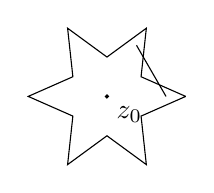
\begin{tikzpicture}[scale = 0.25]
    \draw (0:4) -- (30:2) -- (60:4) -- (90:2) -- (120:4) -- (150:2) -- (180:4) -- (210:2) -- (240:4) -- (270:2) -- (300:4) -- (330:2) -- (360:4);
    \draw[fill] (0,0) circle (0.08);
    \draw node at (0,0) [below right] {$z_0$};
    \draw (0:3) -- (60:3);
\end{tikzpicture}
\end{center}

\begin{remark}
$\oic$ open and star-shaped. Then $\exists z_0 \in \om$ s.t. $\forall z \in \om$, $\overline{z z_0} \subset \om$. Note that $z=z_0 + re^{i \theta} $ for the unique $r = \abs{z-z_0}$ and some unique $\theta$. Parameterize $\overline{z z_0}$ by $\gamma = z_0 + s e^{i \theta}, \, s \in [0,r]$.

Given two paths $\gamma_0 (t), \gamma_1 (t)$ in $\om$, write:
\begin{align*}
\gamma_0(t) &= z_0 + r_0 (t) e^{i \theta_0 (t)}\\
\gamma_1(t) &= z_0 + r_1 (t) e^{i \theta_1 (t)}\\
&\Downarrow\\
\gamma_s(t) &= s_0 + \big( (1-s)r_0(t) + sr_1(t) \big) e^{i \big( (1-s) \theta_0 (t) + s \theta_1 (t) \big)} .
\end{align*}


We may assume that $\gamma_0$ and $\gamma_1$ don't pass through $z_0$ (no proof is given of this fact). Then $\gamma_s$ is a homotopy between $\gamma_0$ and $\gamma_1$ in $\om$.

\end{remark}


\begin{example}[Slit Plane]
Let $\gamma$ be a ray (a closed half-line).
Then $\C \setminus \gamma$ is a slit plane. Up to translation and rotation, we may assume that the slit plane is $\C \setminus \set{(-\infty , 0] }$. This set is star-shaped with respect to the origin, and thus simply connected (but not convex).

\end{example}


\begin{counterexample}
$\C^*$ is not simply connected, as was seen last lecture. Similarly $\DrP{r}{z_0}$ is not simply connected. Similarly any domain with finitely many punctures is not simply connected. Similarly domains with holes that are not just points (such as annuli) are not simply connected.
\end{counterexample}

\begin{note}
Intuitively, a domain with holes is not simply connected, and a domain with no holes is simply connected. This requires algebraic topology beyond the scope of this class to prove.
\end{note}

\subsection{Characterization of Simply Connected Sets}
\begin{theorem}\label{thm:char-simp-conn}
$\oic$ open and connected, $f$ holomorphic on $\om$. Then the following are equivalent:
\begin{enumerate}
    \item $f$ has an antiderivative on $\om$.
    \item $\int_\gamma f(z) \dif z = 0$ $\forall \, \gamma \subset \om$ piecewise smooth closed curve.
    \item $\int_{\gamma_0} f(z) \dif z = \int_{\gamma_1} f(z) \dif z$ $\forall \, \gamma_0, \, \gamma_1 \subset \om$ piecewise smooth curves with same initial and end points.
\end{enumerate}

Furthermore:
\begin{enumerate}
    \item[4.] $\om$ simply connected
\end{enumerate}
implies statements 1, 2, and 3.

\end{theorem}

\begin{remark}
In fact, in the above theorem, statement 1 holding true for all $f$ holomorphic in $\om$ implies statement 4. We will not prove this yet -- it can be proven now using some difficult algebraic topology, but the standard approach in this course is to prove it as a corollary of the Riemann Mapping Theorem (theorem (\ref{thm:r-map-thm})).
\end{remark}

\begin{proof}[\ref{thm:char-simp-conn}]
\begin{enumerate}
    \item[$(4)\Rightarrow (2):$] Already done in corollary (\ref{cor:simp-conn-int-to-zero}).
    \item[$(1)\Rightarrow (2):$] By theorem (\ref{thm:FTC}): $\int_\gamma f(z) \dif z = F(\gamma(b)) - F(\gamma(a)) = F(\gamma(a)) - F(\gamma(a)) = 0$.
    \item[$(2)\Rightarrow (3):$] Given $\gamma_0, \, \gamma_1$, let $\gamma = \gamma_0 \cup -\gamma_1$. Then $\gamma$ is piecewise smooth and closed. By (2):
    \begin{align*}
        0= \int_\gamma f(z) \dif z &= \int_{\gamma_0} f(z) \dif z - \int_{\gamma_1} f(z) \dif z.\\
        &\Downarrow\\
        \int_{\gamma_0} f(z) \dif z &= \int_{\gamma_1} f(z) \dif z.
    \end{align*}
    
    \item[$(3)\Rightarrow (1):$] We must construct $F$ an antiderivative for $f$. Fix $z_0 \in \om$. Given $z \in \om$, since $\om$ is connected we can let $\gamma: [a,b] \to \om$ piecewise smooth with $\gamma(a) = z_0$ and $\gamma(b) = z$.
    
\begin{center}
\begin{tikzpicture}[decoration={
    markings,
    mark=at position 0.5 with {\arrow{>}}}
    ]
    \draw[xshift=50,scale = 0.5] plot [smooth cycle] coordinates {(-10,0) (-7,3.5) (0,5)  (4,4) (7,0)  (5,-5) (2,-6)  (-5,-5) };
    \draw node at (-2,-2) {$\om$};
    \node (a) at (0,0) {};
    \node (b) at (3,-2) {};
    \draw[fill] (a) circle (0.08);
    \draw[fill] (b) circle (0.08);
    \draw (a)+(-0.3,-0.3) node {$z_0$};
    \draw (b)+(0.3,-0.3) node {$z$};
    \draw[postaction = {decorate}] (a) to[out= 0, in = 180] node[midway, below left] {$\gamma$} (b);
\end{tikzpicture}
\end{center}
    
    Define $F(z) \defas \int_\gamma f(w) \dif w$. Note that the LHS doesn't depend on $\gamma$, since by (2) different $\gamma$ yield the same value. Thus this formula above defines a functions $F: \om \to \C$.
    
    
    
    We claim that $F$ is an antiderivative for $f$ on $\om$, ie that $F$ is holomorphic and $F'(z) = f(z) \, \, \forall z \in \om$. Then, with $h$ small such that $D_{\abs{h}} (z) \ssubset \om$, and letting $\sigma$ be a path from $z_0$ to $z+h$:
        \begin{center}
\begin{tikzpicture}[decoration={
    markings,
    mark=at position 0.5 with {\arrow{>}}}
    ]
    \draw[xshift=50,scale = 0.5] plot [smooth cycle] coordinates {(-10,0) (-7,3.5) (0,5)  (4,4) (7,0)  (5,-5) (2,-6)  (-5,-5) };
    \draw node at (-2,-2) {$\om$};
    \node (a) at (0,0) {};
    \node (b) at (3,-2) {};
    \node (c) at (2,1) {};

    \draw[fill] (a) circle (0.08);
    \draw[fill] (b) circle (0.08);
    \draw[fill] (c) circle (0.08);
    
    \draw (a)+(-0.3,-0.3) node {$z_0$};
    \draw (b)+(0.3,-0.3) node {$z$};
    \draw (c)+(0.35,0.3) node {$z+h$};
    
    \draw[postaction = {decorate}] (a) to[out= 0, in = 180] node[midway, below left] {$\gamma$} (b);
    \draw[postaction = {decorate}] (a) to[out= 30, in = 130] node[midway, above left] {$\sigma$} (c);

    
\end{tikzpicture}
\end{center}
    \begin{align*}
        F(z+h) - F(z) &= \int_\sigma f(w) \dif w - \int_\gamma f(w) \dif w\\
        &= \int_{\sigma \cup (- \gamma) } f(w) \dif w\\
        &= \int_{L_z^{z+h}} f(w) \dif w.
    \end{align*}
    
    Recalling that $L_z^{z+h}$ is the line from $z$ to $z+h$.
    
\begin{center}
\begin{tikzpicture}[decoration={
    markings,
    mark=at position 0.5 with {\arrow{>}}}
    ]
    \draw[xshift=50,scale = 0.5] plot [smooth cycle] coordinates {(-10,0) (-7,3.5) (0,5)  (4,4) (7,0)  (5,-5) (2,-6)  (-5,-5) };
    \draw node at (-2,-2) {$\om$};
    \node (a) at (0,0) {};
    \node (b) at (3,-2) {};
    \node (c) at (2,1) {};

    \draw[fill] (a) circle (0.08);
    \draw[fill] (b) circle (0.08);
    \draw[fill] (c) circle (0.08);
    
    \draw (a)+(-0.3,-0.3) node {$z_0$};
    \draw (b)+(0.3,-0.3) node {$z$};
    \draw (c)+(0.35,0.3) node {$z+h$};
    
    \draw[postaction = {decorate}] (b) to[out= 180, in = 0] node[midway, below left] {$\tau$} (a);
    \draw[postaction = {decorate}] (a) to[out= 30, in = 130] node[midway, above left] {} (c);
    \draw[postaction = {decorate}] (b) to[out = 95, in = -80] node[midway, above right] {$L_z^{z+h}$} (c);

    
\end{tikzpicture}
\end{center}
    
    
    
    Thus, remembering that $\frac{1}{h} \int_{L_z^{z+h}} f(w) \dif w = f(z)$ (this was shown in the proof of theorem (\ref{cor:local-prim})):
    \begin{align*}
        \frac{F(z+h) - F(z)}{h} &= \frac{1}{h} \int_{L_z^{z+h}} f(w) \dif w\\
        &= f(z).
    \end{align*}
    
    And we are done, since we have found an antiderivative of $f$ on $\om$.
    
    
    
    
    
\end{enumerate}    

\end{proof}



\section{Complex Logarithm}

We now turn our attention to the question of the complex logarithm. We discovered that there are infinitely many solutions which differ by $2 \pi i k, \, k \in \mathbb{Z}$.

\begin{theorem}\label{thm:complex-log}
$\oic$ open and simply connected, with $0 \not\in \om$, then $\exists F : \om \to \C$ holomorphic (called a \textbf{branch} of the complex logarithm on $\om$) such that:
\begin{align*}
    e^{F(z)} &= z  &\forall z \in \om.
\end{align*}

Furthermore, this $F$ is unique up to adding $2 \pi i k, \, k \in \mathbb{Z}$. That is to say that two different branches differ by an integer multiple of $2 \pi i$.
\end{theorem}

\begin{proof} Let $f(z) = \frac{1}{z}$. This is holomorphic in $\om$ since $0 \not\in \om$. $\om$ is simply connected -- by theorem (\ref{thm:char-simp-conn}) there exists an antiderivative $F(z)$ on $\om$. Note that we can add any complex number to $F$ and still get an acceptable antiderivative. Then:
\begin{align*}
    \left( ze^{-F(z)} \right)' &= e^{-F(z)} - z F'(z) e^{-F(z)}\\
    \text{(since $F'(z) = 1/z$) }&= 0.\\
    &\Downarrow\\
    ze^{-F(z)} &= z_0 \in \C, \: z_0 \neq 0.
\end{align*}

Thus, $e^{F(z)} = \frac{z}{z_0}, \, \forall z \in \om$. Since $z_0 \neq 0$, we can pick $w_0 \in \C$ s.t. $e^{w_0} = z_0$. Then let $\Tilde{F} (z) = F(z) + w_0$. Then:
\begin{align*}
    e^{\Tilde{F} (z)} = e^{F (z)} \cdot e^{w_0} = 1.
\end{align*}


Now assume that $F_1, \, F_2$ are two holomorphic functions on $\om$ which satisfy $e^{F_i(z)} = z$. Then:
\begin{align*}
e^{F_1(z) - F_2(z)} = 1.
\end{align*}
It follows that, since $\set{z \mid e^z = 1} = \set{ 2 \pi i k \mid k \in \mathbb{Z}}$, that:
\begin{align*}
    F_1(z) - F_2(z) = 2 \pi i k(z).
\end{align*}

However the LHS is continuous, so the RHS is too. Since $\mathbb{Z}$ is disconnected, it follows that $k(z)$ is constant. Thus, for some $k \in \mathbb{Z}$:
\begin{align*}
    F_1(z) - F_2(z) = 2 \pi i k.
\end{align*}

\end{proof}


\begin{remark}
In theorem (\ref{thm:complex-log}), if furthermore $1 \in \om$, then letting $z_0 = 1$ in the above proof, and adding a constant to $F$ such that $F(1) = 0$ we get that $ze^{-F(z)} = z_0$. evaluating now at $z=1$, we get $z_0 = 1$. Thus $\Tilde{F} = F$ and $\Tilde{F} (1) = 0$.\\

This is called the \textbf{principal branch of $\mathbf{log}$}, denoted by $\log(z)$, with the property that $\log(1) = 0$.
\end{remark}

